\documentclass[11pt,letterpaper]{article}
\usepackage{samstyle}

\title{Brocken Data Base:BRKDB}
        
\author{
	Profesor\\
	Sergio Andres Monsalve Castañeda\\
	smonsal3@eafit.edu.co
}

\begin{document}
 
\pagestyle{fancyplain}
\fancyhf{}
\headheight=20pt %para cambiar el tamaño del encabezado
\renewcommand{\headrulewidth}{0pt} %espesor del encabezado

% \lhead %la "L" indica a la izquierda
% {
% }

\fancyfoot[c]{\thepage}

\maketitle

\begin{minipage}{3cm}
% 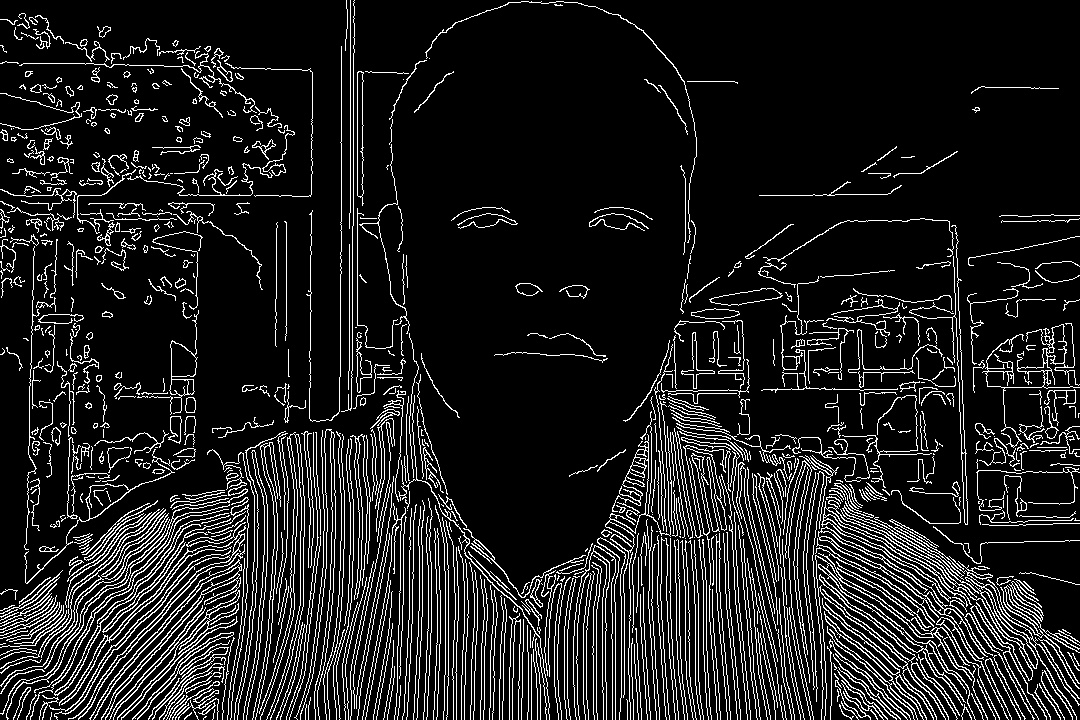
\includegraphics[width=15cm]{aux/SamCanny.jpg}
\end{minipage}


\section{Description}

A university course database has brocken, one of the colums has been completely deleted and that column had the names of the 3 students that belong to that gruop. It is know that in that course where only 3 students with the same surnename and diferent lastnames and diferent id codes.
You have the following data: ``Monsalve'' had the code 200410061010, ``Silva'' had 200120039010 and ``Pineda'' 199810043010.

Your goal is to get back the data base integrity and print the surenames, lastnames and codes of the students one per line. 


\section{Input}

As input read the name that had been deleted and now has been recovered by the IT personal of the university.

\section{Output}

It is expected that your problem prints as outputs one line per person replaced with the given data:

Name + space +  Lastname1 + space + code1 \\
Name + space +  Lastname2 + space + code2 \\
Name + space +  Lastname3 + space + code3 \\

\section{Example}
\subsection{Input}
\lstinputlisting{db.in}
\subsection{Output}
\lstinputlisting{db.ot}

%\bibliographystyle{plainnat}
%\bibliography{refs}

\end{document}


